\section{Centre, frontière et vacances dans la connexion nonadique}
\label{sec:centro-frontera}
\subsection{La thèse et l'ordre de construction}
La relation entre centre et frontière acquiert un contenu mathématique lorsque l'on précise quelles données sont exprimées, quelles transformations les transportent et à l'aide de quelles informations on les reconstruit. Dans APP, un résidu s'accompagne de son quotient ; dans TRIT, l'orientation distingue des opérations qu'un agrégat peut réunir ; dans TPK, un tour ramène la phase et prolonge la mémoire. L'état enrichi réunit ces coordonnées. Son inscription dans la structure discrète conjointe du continu conserve les dépendances entre les différentes lectures ultérieures.

Le parcours est APP → TRIT → TPK → état enrichi → structure discrète conjointe du continu. Ce développement effectue des coupes locales de ce parcours : il ne reconstruit pas les cinq aspects consubstantiels du continu à partir d'une forme spectrale et ne les transforme pas en cinq modules indépendants. Les constantes internes sont reçues à leur stade de représentation, sans utiliser leurs valeurs conventionnelles pour choisir des germes, des parcours ou des coefficients.

L'intuition de l'auteur peut s'exprimer ainsi : \textbf{la représentation d'une valeur est une projection d'une construction ; pour transporter cette construction, on conserve l'information qui permet de distinguer ses réalisations}. Les opérations suivantes concrétisent cette affirmation. Le langage ultérieur de l'interpolation et de la décomposition orthogonale démontre des propriétés d'objets déjà spécifiés ; il ne sélectionne pas rétrospectivement l'état APP.

\subsection{La couronne locale et la reconstruction du centre}
Dans la coordinatisation positive, on utilise

\[
\rho_9(n)=1+[(n-1)]_9,\qquad
q_9(n)=\frac{n-\rho_9(n)}9,
\qquad n=\rho_9(n)+9q_9(n).
\]
La table du produit est \(P(i,j)=ij\), avec \(1\leq i,j\leq9\). La restriction à \(Q=\{3,4,5,6\}^2\) exprime

\[
\left(\rho_9(ij)\right)_{i,j=3}^{6}=
\begin{pmatrix}
9&3&6&9\\
3&7&2&6\\
6&2&7&3\\
9&6&3&9
\end{pmatrix}.
\]
\begin{figure}[htbp]
\centering
\begin{minipage}[c]{.46\textwidth}
\centering
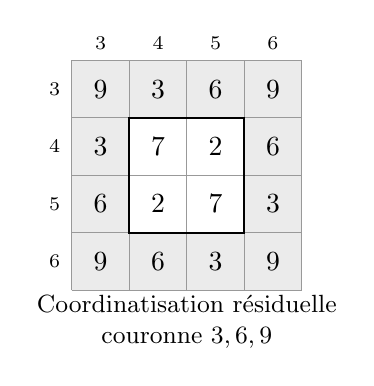
\begin{tikzpicture}[x=.73cm,y=.73cm]
\fill[black!8] (0,0) rectangle (4,4);
\fill[white] (1,1) rectangle (3,3);
\draw[step=1,black!40] (0,0) grid (4,4);
\draw[thick] (1,1) rectangle (3,3);
\foreach \row/\vals in {0/{9,3,6,9},1/{3,7,2,6},2/{6,2,7,3},3/{9,6,3,9}}{
  \foreach \val [count=\col from 0] in \vals{
    \node at (\col+.5,3.5-\row) {\(\val\)};
  }
}
\foreach \v [count=\n from 0] in {3,4,5,6}{
  \node[font=\scriptsize] at (\n+.5,4.3) {\(\v\)};
  \node[font=\scriptsize] at (-.3,3.5-\n) {\(\v\)};
}
\node[font=\small,align=center] at (2,-.55) {Coordinatisation résiduelle\\couronne \(3,6,9\)};
\end{tikzpicture}
\end{minipage}\hfill
\begin{minipage}[c]{.50\textwidth}
\centering
\begin{tikzpicture}[x=.73cm,y=.73cm]
\fill[black!3] (0,0) rectangle (4,4);
\draw[black!40] (0,0) rectangle (4,4);
\draw[thick] (1,1) rectangle (3,3);
\foreach \x/\y/\v in {.5/3.5/9,3.5/3.5/18,.5/.5/18,3.5/.5/36,
  1.5/2.5/16,2.5/2.5/20,1.5/1.5/20,2.5/1.5/25}{
  \node at (\x,\y) {\(\v\)};
}
\draw[-{Stealth},black!60] (.85,3.15) -- (1.22,2.78);
\draw[-{Stealth},black!60] (3.15,3.15) -- (2.78,2.78);
\draw[-{Stealth},black!60] (.85,.85) -- (1.22,1.22);
\draw[-{Stealth},black!60] (3.15,.85) -- (2.78,1.22);
\node[font=\small,align=center] at (2,-.55) {Frontière relevée\\et interpolation multiaffine};
\end{tikzpicture}
\end{minipage}
\caption{La même coordinatisation selon deux lectures. À gauche, la couronne radicale entoure le bloc \(B_c\). À droite, les quatre sommets entiers déterminent les valeurs intérieures sous la loi multiaffine. Leurs résidus aux sommets coïncident, mais les quotients \((0,1,1,3)\) distinguent le relèvement.}
\label{fig:centro-frontera}
\end{figure}


\Needspace{6\baselineskip}
Son bloc intérieur est

\[
B_c=\begin{pmatrix}7&2\\2&7\end{pmatrix}.
\]
Le périmètre de cette coordinatisation contient douze positions : quatre de valeur \(3\), quatre de valeur \(6\) et quatre de valeur \(9\) ; leur somme est \(72\). Une couronne radicale apparaît autour du bloc central. Le centre électronique global est \((5,5)\), unique point fixe de l'inversion de l'APP complète ; sa position ne change pas lorsque l'on choisit cette coordinatisation locale, dont le centre géométrique se trouve en \((4.5,4.5)\).

\begin{proposition}[Récupération à partir de la frontière relevée]
\label{prop:centro-frontera-recuperacion}
Soit \(F(x,y)=a+bx+cy+dxy\) une loi multiaffine dans la coordinatisation \([3,6]^2\). Pour \(t=(x-3)/3\) et \(u=(y-3)/3\),

\[
\begin{aligned}
F(x,y)={}&(1-t)(1-u)F(3,3)+(1-t)uF(3,6)\\
&+t(1-u)F(6,3)+tuF(6,6).
\end{aligned}
\]
\end{proposition}
\begin{proof}
Pour \(y\) fixé, le caractère affine en \(x\) permet de retrouver \(F(x,y)\) à partir de \(F(3,y)\) et de \(F(6,y)\). Le caractère affine en \(y\) permet de retrouver chacune de ces deux valeurs à partir de ses extrémités. La composition donne la formule. En particulier, les quatre sommets déterminent toute la coordinatisation dans l'espace de lois déclaré.
\end{proof}

Pour le produit, les quatre valeurs relevées sont \(9,18,18,36\). Leurs résidus positifs valent tous \(9\), mais leurs quotients sont \(0,1,1,3\). La formule retrouve \(16,20,20,25\) aux positions intérieures ; leur représentation résiduelle donne \(7,2,2,7\). Ainsi, la frontière détermine l'intérieur \textbf{en conservant la loi et le relèvement}. L'interpolation s'effectue avant la réduction modulaire : on ne divise pas par \(3\) dans \(\mathbb Z/9\mathbb Z\), où \(3\) n'est pas inversible.

Cela précise le sens de « conserver l'information du centre ». La couronne résiduelle seule n'individualise pas tous les relèvements : \(F\) et \(F+9\) ont les mêmes résidus sur toute la frontière et des valeurs relevées distinctes. La paire résidu–quotient élimine cette ambiguïté dans la reconstruction indiquée. L'affirmation est prouvée pour les lois multiaffines ; l'étendre aux états complets exige de conserver également les opérateurs, les routes et la mémoire qui agissent sur eux.

La récupération multiaffine est une \textbf{formalisation nouvelle de l'architecture préexistante de l'auteur}. Les coordinatisations et leurs lectures sont des résultats récupérés dans le corpus ; cette présentation explicite de leur inverse n'est pas attribuée à une découverte historique indépendante.

\subsection{Somme, produit et les trois valeurs de la courbure discrète}
Les lignes multiplicatives sont construites par accumulation additive. La différence entre les deux feuillets apparaît lorsque les deux coordonnées varient simultanément. Avec des différences unitaires,

\[
\Delta_x\Delta_y(x+y)=0,
\qquad
\Delta_x\Delta_y(xy)=1.
\]
La même propriété se retrouve à la frontière relevée :

\[
\frac{P(6,6)-P(6,3)-P(3,6)+P(3,3)}{3\cdot3}=1;
\]
pour \(S(x,y)=x+y\), ce quotient vaut \(0\). Le produit enregistre la variation croisée que la somme n'introduit pas. Le corpus exprime la version orientée par

\[
\mathcal F(T_x,T_y)=\Delta_x\Delta_yT_y-\Delta_y\Delta_xT_x,
\]
\[
\mathcal F(S,S)=\mathcal F(P,P)=0,
\qquad \mathcal F(S,P)=+1,
\qquad \mathcal F(P,S)=-1.
\]
L'ordre des feuillets distingue le signe. La formulation « la somme accumule et le produit plie ou déplie » repose ici sur une opération vérifiable : lors de la projection modulaire, un résidu est conservé ; lors du relèvement, on restitue le quotient qui enregistre le dépassement. La courbure discrète enregistre en outre l'ordre des variations. Cette différence finie n'est pas identifiée à une courbure différentielle d'un espace physique sans son application de réalisation correspondante.

\subsubsection*{La croix radicale globale}
Dans \(R=\mathbb Z/9\mathbb Z\), l'idéal \(\mathfrak m=\{0,3,6\}\) satisfait \(\mathfrak m^2=0\). Sa représentation positive est \(\{9,3,6\}\). La croix

\[
(\mathfrak m\times R)\cup(R\times\mathfrak m)
\]
comporte \(27+27-9=45\) positions. L'intersection contient neuf valeurs \(9\), de somme \(81\) ; les bras restants contiennent douze valeurs de chaque classe \(3,6,9\), de somme \(216\). Le total est

\[
297=216+81=3(72+27)=3\cdot99.
\]
On distingue quatre frontières : le périmètre local de douze positions, la croix radicale de quarante-cinq, le gnomon de dix-sept qui complète \(8^2\) en \(9^2\), et la couronne cubique de \(271\). Chacune possède son propre domaine et sa propre opération. Le quotient tritique \(R/\mathfrak m\) conserve une classe ; transporter l'état exige de l'accompagner des données relevées et de son histoire.

\subsection{Les lecteurs 72–27, 77–22 et la complétion 729–271}
Les lignes ordonnées de \(B_c\) s'expriment en écriture décimale par \(72\) et \(27\) ; leurs diagonales par \(77\) et \(22\). Il en résulte

\[
72+27=77+22=99.
\]
Dans la complétion cubique, le dénombrement de l'intérieur, des faces, des arêtes et du sommet donne

\[
1000=729+243+27+1=729+271,
\]
\[
999=729+243+27=729+270.
\]
La coïncidence des lecteurs s'exprime en conservant le reste décimal :

\[
729=10\cdot72+9,\qquad271=10\cdot27+1.
\]
Ainsi, la lecture bidimensionnelle exprime \((72,27)\) ; la lecture cubique exprime \(((72,9),(27,1))\). Le couple de restes \((9,1)\) distingue les prolongements qui partageraient un même quotient. On effectue d'abord les constructions des coordinatisations ; on compare ensuite ces représentations. L'identité des entiers n'inverse pas cet ordre causal.

Le chapitre des canaux entiers fournit une autre composition spécifique. Avec les dénombrements internes \(\Delta=54\), \(\nu=\Delta/2=27\) et \(\Theta=5\nu=135\), il obtient

\[
\mathcal C_\alpha=\nu^2=729,
\qquad \mathcal C_e=2\Theta+1=271.
\]
On a renommé ici \(\nu\) l'entier local que ce propriétaire écrit \(\kappa\), pour le distinguer de la lecture rationnelle du registre dodécaphasique. Les canaux sont des objets entiers ; leur identification aux constantes passe par les lecteurs régionaux et la clôture correspondante, et non par les premiers chiffres d'un développement. Cette comparaison utilise les canaux entiers et n'a pas besoin de la réalisation angulaire ultérieure.

Pour la référence orale à une fraction de \(\pi\), le propriétaire localisé contient

\[
\frac{396}{126}=\frac{22}{7},\qquad
396=18+72+108+198,\quad126=18+108.
\]
Il s'agit d'un rapport rationnel d'anneaux alternés. Ce rapport d'anneaux est une lecture rationnelle exacte ; sa fonction se distingue de la représentation régionale de \(\pi\).

\subsection{Le centre électronique et ses vacances conjuguées}
L'inversion de l'APP positive est \(\rho(r,c)=(10-r,10-c)\). Son unique point fixe est \((5,5)\). Dans la fibre additive centrale,

\[
\mathcal F_{10}=\{(5+t,5-t):t\in\mathbb Z,\ |t|\leq4\},
\]
le produit vaut \(25-t^2\). Conserver son résidu central exige \(t^2\equiv0\pmod9\), équivalent à \(3\mid t\). Les seuls emplacements sont donc

\[
(5,5),\qquad(8,2),\qquad(2,8).
\]
Si \(\mathcal A\) conserve la paire résidu–quotient dans chaque feuillet,

\[
\begin{aligned}
\mathcal A(5,5)&=((1,1),(7,2)),\\
\mathcal A(8,2)=\mathcal A(2,8)&=((1,1),(7,1)).
\end{aligned}
\]
Les deux vacances préservent la lecture additive et le résidu multiplicatif ; le quotient du produit diminue exactement d'une unité. Le miroir \(t\mapsto-t\) échange leurs positions. La valeur résiduelle ne distingue pas leurs routes, tandis que l'orientation les conserve. C'est une réalisation précise de la connexion indiquée par la note : \textbf{la vacance s'individualise par une relation au centre et par un défaut enregistré, et non parce qu'elle serait une case sans information}.

L'orientation électronique initiale \((h_0,v_0)=(1,1)\), inversée tous les \(27\) pas, exprime ensuite la signature dodécaphasique \((+++\,---\,+++\,---)\). Il s'agit d'un registre d'orientation, distinct tant de la position \((5,5)\) que de la signature de produit suivante.

\subsubsection*{La signature 555555 et la mémoire qui permet de la prolonger}
Pour \(U_j=100d_{1j}+10d_{2j}+d_{3j}\), le lecteur

\[
\mathcal E_\times(U)=([d_{2j}-d_{1j}]_{10})_{j=1}^{6}
\]
appliqué à la région transversale

\[
U_\pi^\perp=(501,614,498,169,272,272)
\]
produit \(555555\) ; sa réduction \(\Psi(U)=(-U_j\bmod3)_j\) produit \(010211\). La signature possède vingt-quatre représentants produit. Le transport les sépare en trois feuillets de huit : après l'avancée apparaissent \(555177\), \(555717\) et \(555771\). La congruence stable par avancée et demi-tour raffine les vingt-six signatures en vingt-huit classes, d'histogramme \(27\cdot8+108=324\). Cela exprime pourquoi il faut retenir une mémoire de feuillet pour poursuivre une signature qui coïncide initialement.

\begin{definition}[Lecteur de signature et transport des représentants]
\label{def:firma555}
Soit \(\mathcal X_\times=D_9^2\times\{N,E,S,O\}\), de cardinal \(324\).
L'avancée \(P\) déplace d'une case dans la direction mémorisée et le demi-
tour \(H\) inverse cette direction. Le lecteur utilise
\[
\ell_9(1,2,4,8,7,5)=(0,1,2,3,4,5),\qquad
\ell_9(3)=\ell_9(6)=\ell_9(9)=0.
\]
Dans chacune des six fenêtres de neuf étapes, on évalue
\(\ell_9(\rho_9(ij))\) avant l'avancée produit sélectionnée par TRIT aux
temps \(2,5,8\pmod9\). La somme de chaque fenêtre est réduite modulo
\(10\). Après les étapes \(27\) et \(54\), la direction est inversée.
La règle détermine \(E_{\rm sig}(x)\) à partir de la position et de la direction
de \(x\), avec les conventions temporelles du noyau.
\end{definition}

\begin{proposition}[Raffinement minimal stable de la signature]
\label{prop:firma555}
En partant de l'équivalence par signature \(\sim_0\), l'itération
\[
x\sim_{n+1}y\ \Longleftrightarrow\
x\sim_n y,\quad Px\sim_n Py,\quad Hx\sim_n Hy
\]
se termine et produit la congruence stable la plus grossière qui raffine la signature. Dans le domaine précédent, le recensement est \(26\to28\to28\) ; la fibre de \(555555\) se sépare en trois classes de huit représentants.
\end{proposition}
\begin{proof}
À chaque étape, on raffine une partition d'un ensemble fini. Le processus se
stabilise après un nombre fini de scissions. Au point fixe,
l'équivalence est préservée sous \(P\) et \(H\). Si une congruence stable
raffine \(\sim_0\), elle raffine par récurrence chaque \(\sim_n\) : ses images
par les deux opérateurs restent équivalentes. Elle raffine donc le point
fixe obtenu, ce qui prouve sa minimalité en information ajoutée.

L'énumération finie applique la définition aux \(81\) positions et aux quatre orientations. On regroupe d'abord leurs six sommes modulo \(10\), puis le triplet formé par la classe de \(x\), celle de \(Px\) et celle de \(Hx\), jusqu'à stabilisation. L'histogramme résultant est \(27\cdot8+108=324\), et la seule scission de signature est celle indiquée. Les représentants suivants explicitent les trois images :
\[
\begin{array}{c|c|c}
x&E_{\rm sig}(x)&E_{\rm sig}(Px)\\\hline
(3,5,N)&555555&555177\\
(3,4,N)&555555&555717\\
(3,4,S)&555555&555771
\end{array}
\]
La règle complète et son énumération exécutable sont conservées dans le paquet
de reproduction ; les témoins du tableau montrent en outre que conserver
seulement la signature ne rend pas sa continuation univoque.
\end{proof}

La conclusion décrit l'information minimale du transport, et non une
nouvelle masse. Le facteur additif conserve dix-huit représentants par signature
(neuf positions compatibles et deux orientations). En le combinant avec les
fibres produit de tailles \(24\) et \(8\), on obtient respectivement
\(432\) et \(144\). L'incidence régionale et la mémoire de feuillet conservent
ainsi des fonctions distinctes dans le même catalogue.


Le lien avec l'équation électronique passe par les régions. La région transversale a pour multiplicité \(432=18\cdot24\) ; chacune des quatre autres a \(144=18\cdot8\). Leurs cinq identités s'insèrent, dans la jauge déclarée de l'article I, dans

\[
\mathcal K_e=\mathbb Z/9\mathbb Z\times\mathbb F_3
\]
au moyen de \((4,0),(5,0),(6,0),(6,1),(6,2)\). Une fois cette insertion fixée, son complément comporte \(27-5=22\) places et ses trois feuillets par région comportent \(5\cdot3=15\) places. Le déficit orienté et la mémoire torsionnelle sont \(-22\) et \(15\). La preuve de ces dénombrements s'obtient à partir de l'injection explicite précédente : ses cinq images sont distinctes ; ce développement la rassemble et ne choisit pas ses places à partir d'une masse cible.

Il y a donc deux parcours liés dans la composition : \textbf{centre → vacances conjuguées → orientation}, et \textbf{signature régionale → feuillets de transport → incidence des cinq régions → coefficients électroniques}. Identifier sans autre précision \((5,5)\) à \(555555\) effacerait précisément les opérations qui expliquent leur relation.

\subsection{Miroir nonadique, capacité et retour à mémoire}
Dans la fibre régionale, le miroir agit par

\[
\mathfrak c(u^\pi,u^e,u^\varphi)=(u^e,u^\pi,u^\varphi).
\]
Il conserve \(s=u^\pi+u^e\) et inverse \(d=u^\pi-u^e\). En \(\mathbb F_3\),

\[
u^\pi=2(s+d),\qquad u^e=2(s-d).
\]
La somme conserve l'agrégat ; la différence orientée conserve la répartition. L'axe \(u^\varphi\) reste fixe sous cette involution, bien qu'il puisse évoluer sous le transport. Le miroir régional et le miroir cellulaire des vacances ont des domaines distincts : leurs formules respectives permettent de suivre ce que chacun préserve.

La vacance de capacité ajoute un lien temporel explicite. Dans la normalisation du raffinement \(729\) par rapport à \(1000\), soient \(\rho_c=\log_{10}9\), \(\delta=1-\rho_c\) et \(\mathcal C_t=\lfloor(t+1)\rho_c\rfloor\). Si

\[
z_t=\lfloor(t+1)\delta\rfloor-\lfloor t\delta\rfloor,
\]
alors, pour \(t\geq1\),

\[
\mathcal C_t-\mathcal C_{t-1}=1-z_t,
\qquad
\mathcal C_b-\mathcal C_a+\sum_{t=a+1}^b z_t=b-a.
\]
\begin{proof}
L'irrationalité de \(\log_{10}9\) découle de l'impossibilité de \(9^n=10^m\) pour des entiers positifs. Par conséquent, \(\mathcal C_t=t-\lfloor(t+1)\delta\rfloor\). Soustraire et sommer télescopiquement donne les deux identités. \end{proof}
Une vacance retient la capacité tandis que l'histoire avance.

Si \(p_j=\lfloor j/\delta\rfloor\), \(v_j=p_j-j\) et \(h_j=p_{j+1}-p_j\), le développement hérité établit \(h_j\in\{21,22\}\). Pour \(s_j=22-h_j\),

\[
[v_{j+1}]_3=[v_j-s_j]_3,\qquad
\tau_j=M_{\rm ph}(1+[v_j]_9).
\]
Les vacances agissent ainsi sur la phase retenue que lit le sélecteur tritique. Cette suite de capacité ne devient pas automatiquement la trajectoire cellulaire de l'électron : le manuscrit conserve leurs mécanismes respectifs et leur composition dans le même noyau.

% RESULTADO_RECUPERADO y exposición autónoma ampliada; no cambia el núcleo común.
% Propietarios cotejados:
% Artículo I REV02/sections/vacancias_capacidad.tex, completo.
% Monografía775/manuscrito/generated/cristal_relojes_sincronizacion.tex,
% líneas1--223 y931--1032: capacidad, retornos e inducción TRIT.
% Las pruebas universales de las dos escalas se reúnen aquí; el comprobador
% ampliacion/verificar_vacancias.py añade un certificado racional finito.
\subsection{Vacances du raffinement nonadique et hiérarchie des retours}
\label{vac-add-seccion}

Le prolongement APP--TRIT--TPK conserve, avec le bloc exprimé, le cylindre, l'orientation et l'historique qui permettent de le poursuivre. Dans sa lecture de capacité, on compare deux cardinaux déjà déterminés par cette construction : les \(3^6=729\) possibilités d'un bloc ternaire à six positions et les \(10^3=1000\) positions de sa coordinatisation décimale à trois chiffres. Cette comparaison produit un calendrier propre. Certaines transitions augmentent l'indice de capacité ; d'autres incorporent un bloc à l'historique tout en maintenant cet indice. Ces dernières sont les \emph{vacances de capacité} étudiées ci-dessous.

L'objet considéré est donc une représentation du raffinement conjoint. Sa définition conserve l'origine dans les deux supports finis ; l'expression logarithmique permet de démontrer les propriétés de son calendrier. Le temps de bloc, l'indice de vacance et l'indice de capacité seront écrits séparément. Cette séparation rend visible la raison pour laquelle les retours \(21/22\) et \(6/7\) appartiennent à des échelles successives d'une même construction.

\subsubsection{Capacité décimale et conservation de l'incrément}
\label{vac-add-capacidad}

\begin{definition}[Indice de capacité et vacance]
\label{vac-add-definicion}
À l'origine de phase \(0\), on définit
\begin{equation}
 \rho=\log_{1000}729=\log_{10}9,
 \qquad \delta=1-\rho=\log_{10}(10/9),
 \label{vac-add-densidad}
\end{equation}
et, pour \(t\in\mathbb Z_{\geq0}\),
\begin{equation}
 \mathcal C_t=\lfloor(t+1)\rho\rfloor,
 \qquad
 z_t=\lfloor(t+1)\delta\rfloor-\lfloor t\delta\rfloor.
 \label{vac-add-indices}
\end{equation}
L'entier \(\mathcal C_t\) est l'indice de capacité décimale du lecteur ;
\(z_t=1\) indique une vacance. La lettre \(K\) demeure réservée au
registre dodécaphasique et ne désigne pas ici un compteur de capacité.
\end{definition}

On a \(0<\delta<1\). En outre, \(\delta\) est irrationnel : si \(\rho=a/b\) était rationnel, avec \(a,b\) entiers positifs, l'égalité \(9^b=10^a\) aurait une valuation nulle au nombre premier \(5\) à gauche et positive à droite. Cette contradiction démontre l'irrationalité de \(\rho\) et de \(1-\rho\). En particulier, aucun multiple entier positif de \(\delta\) n'appartient à \(\mathbb Z\), ce qui fixe sans ambiguïté les extrémités des intervalles de ce développement.

\begin{proposition}[Bilan exact de capacité et de vacance]
\label{vac-add-balance}
Pour \(t\geq1\), \(z_t\in\{0,1\}\) et
\begin{equation}
 \mathcal C_t-\mathcal C_{t-1}=1-z_t.
 \label{vac-add-incremento}
\end{equation}
Par conséquent, pour \(0\leq a<b\),
\begin{equation}
 \mathcal C_b-\mathcal C_a+
 \sum_{t=a+1}^{b}z_t=b-a.
 \label{vac-add-conservacion}
\end{equation}
\end{proposition}
\begin{proof}
Comme \(0<\delta<1\), la différence entre les parties entières de deux
nombres séparés par \(\delta\) vaut \(0\) ou \(1\). D'autre part,
l'irrationalité démontrée donne
\[
 \mathcal C_t=t+1-\lceil(t+1)\delta\rceil
             =t-\lfloor(t+1)\delta\rfloor.
\]
La soustraction de cette égalité en \(t\) et en \(t-1\) prouve
\eqref{vac-add-incremento} ; sa somme télescopique prouve
\eqref{vac-add-conservacion}.
\end{proof}

Chaque transition apporte exactement une unité au membre de droite du
bilan. Cette unité est enregistrée comme capacité acquise lorsque
\(z_t=0\), ou comme vacance lorsque \(z_t=1\). La rétention de l'indice
\(\mathcal C_t\) laisse donc une position récupérable dans l'
histoire. L'équation exprime la conservation de l'incrément avec deux
lectures, et non une perte indéterminée d'information.

La densité se déduit également du même bilan :
\[
 \frac1N\sum_{t=1}^{N}z_t
 =\frac{\lfloor(N+1)\delta\rfloor}{N}\longrightarrow\delta.
\]
Ainsi, \((z_t)\) n'est pas ultimement périodique : une suite binaire
ultimement périodique possède une densité rationnelle. L'apériodicité
résulte ici de la règle de capacité déjà fixée par \(729/1000\).

\subsubsection{Détermination exacte des intervalles \(21/22\)}
\label{vac-add-primarios}

\begin{lemma}[Bornes rationnelles de la pente]
\label{vac-add-cotas}
La densité de vacance satisfait
\begin{equation}
 \frac7{153}<\delta<\frac6{131}.
 \label{vac-add-cota-delta}
\end{equation}
Si \(\lambda=\delta^{-1}\), \(\beta=22-\lambda\) et
\(\mu=\beta^{-1}\), alors
\begin{equation}
 21<\lambda<22,
 \qquad \frac17<\beta<\frac16,
 \qquad 6<\mu<7.
 \label{vac-add-cotas-inducidas}
\end{equation}
\end{lemma}
\begin{proof}
On fournit une vérification finie par arithmétique rationnelle. Pour \(0<u<1\), soient
\[
 S_N(u)=2\sum_{k=0}^{N}\frac{u^{2k+1}}{2k+1},
 \qquad
 R_N(u)=\frac{2u^{2N+3}}{(2N+3)(1-u^2)}.
\]
L'intégration de la série géométrique de \(2/(1-u^2)\) donne
\[
 S_N(u)<\log\frac{1+u}{1-u}<S_N(u)+R_N(u).
\]
En effet, la queue est positive et, en remplaçant chaque dénominateur
\(2k+1\) par \(2N+3\), elle est bornée par la série géométrique qui
définit \(R_N\). On applique ces inégalités à
\(u=1/19,1/3,1/9\), qui correspondent respectivement à
\(\log(10/9),\log2,\log(5/4)\), et l'on utilise
\(\log10=3\log2+\log(5/4)\).

Avec \(N=4\), en écrivant \(A=S_4(1/19)\), \(B=3S_4(1/3)+S_4(1/9)\) et \(E=3R_4(1/3)+R_4(1/9)\), on obtient
\[
 \frac7{153}
 <\frac{A}{B+E}
 <\delta
 <\frac{A+R_4(1/19)}{B}
 <\frac6{131}.
\]
Les deux inégalités extérieures se vérifient en multipliant par les
dénominateurs positifs de ces sommes de cinq termes rationnels.
On prouve ainsi \eqref{vac-add-cota-delta} au moyen d'une borne du reste,
sans utiliser un développement décimal comme prémisse. En l'inversant, on obtient
\(131/6<\lambda<153/7\). Soustraire à \(22\), puis inverser,
produit toutes les inégalités de \eqref{vac-add-cotas-inducidas}.
\end{proof}

\begin{theorem}[Positions et séparations des vacances]
\label{vac-add-teorema-primario}
Les positions des événements \(z_t=1\), ordonnées à partir du premier événement, sont exactement
\begin{equation}
 p_j=\lfloor j\lambda\rfloor
     =\left\lfloor\frac j\delta\right\rfloor,
 \qquad j\geq1.
 \label{vac-add-posiciones}
\end{equation}
Leurs séparations satisfont
\begin{equation}
 h_j=p_{j+1}-p_j\in\{21,22\}.
 \label{vac-add-huecos}
\end{equation}
Les deux valeurs apparaissent une infinité de fois.
\end{theorem}
\begin{proof}
L'événement qui franchit l'entier \(j\) se produit précisément lorsque
\(t\delta<j<(t+1)\delta\). L'irrationalité exclut l'égalité aux
extrémités. En divisant par \(\delta\), on obtient
\(t=\lfloor j/\delta\rfloor=p_j\). Comme \(\delta<1\), une étape
franchit au plus un entier, de sorte que l'énumération est exacte.
En écrivant \(\lambda=21+\eta\), avec \(0<\eta<1\), on obtient
\[
 h_j=21+\lfloor(j+1)\eta\rfloor-\lfloor j\eta\rfloor,
\]
ce qui prouve \eqref{vac-add-huecos}. Enfin, \((p_{J+1}-p_1)/J\to\lambda\in(21,22)\). Si l'une des deux valeurs n'apparaissait qu'un nombre fini de fois, cette moyenne convergerait vers l'autre valeur entière, ce qui est une contradiction.
\end{proof}

\subsubsection{Induction sur les intervalles courts : les retours \(6/7\)}
\label{vac-add-secundarios}

\begin{theorem}[Calendrier induit des intervalles courts]
\label{vac-add-teorema-secundario}
Soit \(s_j=22-h_j\), pour \(j\geq1\). Cette indicatrice vaut \(1\) exactement lorsque l'intervalle entre vacances est court, de longueur \(21\). Avec \(\beta\) et \(\mu\) définis dans le lemme~\ref{vac-add-cotas},
\begin{equation}
 s_j=\lfloor(j+1)\beta\rfloor-\lfloor j\beta\rfloor.
 \label{vac-add-indicador-corto}
\end{equation}
Les indices des intervalles courts sont
\begin{equation}
 q_m=\lfloor m\mu\rfloor=\lfloor m/\beta\rfloor,
 \qquad q_{m+1}-q_m\in\{6,7\},\quad m\geq1.
 \label{vac-add-posiciones-cortos}
\end{equation}
Les deux séparations se présentent une infinité de fois et leur ordre n'est pas
ultimement périodique.
\end{theorem}
\begin{proof}
L'irrationalité de \(\delta\) implique celle de \(\lambda\),
de \(\beta\) et de \(\mu\). Puisque \(\lambda=22-\beta\), pour
\(j\geq1\), on a
\[
 p_j=22j-\lceil j\beta\rceil
     =22j-\lfloor j\beta\rfloor-1.
\]
En soustrayant des termes consécutifs apparaît
\eqref{vac-add-indicador-corto}. En appliquant à l'indicatrice de pente
\(\beta\) l'argument de franchissement des entiers du théorème précédent,
son événement \(m\) se trouve en \(q_m=\lfloor m/\beta\rfloor\).
L'inégalité \(6<\mu<7\) prouve les deux séparations possibles.
Leur moyenne converge vers \(\mu\) ; elles apparaissent donc toutes deux une infinité
de fois. De plus, une suite de séparations ultimement périodique
aurait une moyenne rationnelle, alors que \(\mu\) est irrationnel. Cela exclut
également une alternance stricte, dont la moyenne serait \(13/2\).
\end{proof}

Les nombres \(6\) et \(7\) comptent ici des \emph{intervalles entre événements de vacance}, et non des blocs de raffinement. Le retour à l'échelle primaire est tout aussi explicite. Entre \(q_m\) et \(q_{m+1}\), il n'y a qu'un seul intervalle court, situé au début, et tous les autres sont longs. Par conséquent, si \(d_m=q_{m+1}-q_m\),
\begin{equation}
 p_{q_{m+1}}-p_{q_m}=21+22(d_m-1)=22d_m-1
 \in\{131,153\}.
 \label{vac-add-retorno-bloques}
\end{equation}
Ainsi, \(131=14\cdot9+5\) et \(153=17\cdot9\) décrivent deux lectures
de retour \emph{dans l'horloge des blocs}. L'équation conserve l'
opération qui relie les échelles, au lieu d'identifier leurs
cardinaux par leur seule apparition.

\subsubsection{Capacité retenue et sélection du régime TRIT}
\label{vac-add-regimen}

Soit \(v_j=\mathcal C_{p_j}\) la capacité enregistrée à la vacance
\(j\). De \(p_j\delta<j<(p_j+1)\delta\) et de \(\delta<1\) résulte
\(\lfloor(p_j+1)\delta\rfloor=j\). D'après
\eqref{vac-add-indices},
\begin{equation}
 v_j=p_j-j,
 \qquad v_{j+1}-v_j=h_j-1=21-s_j,
 \qquad [v_{j+1}]_3=[v_j-s_j]_3.
 \label{vac-add-transporte-mod3}
\end{equation}
Un intervalle long conserve la classe modulo \(3\) ; un intervalle court la décale d'une unité dans le sens négatif. En appliquant le sélecteur du noyau formel à la phase positive \(r_j=1+[v_j]_9\), on obtient
\begin{equation}
 \tau_j=M_{\rm ph}(r_j),\qquad
 M_{\rm ph}(r)=
 \begin{cases}
 +1,&r\in\{1,4,7\},\\
 -1,&r\in\{2,5,8\},\\
 0,&r\in\{3,6,9\}.
 \end{cases}
 \label{vac-add-selector}
\end{equation}
Cette composition fixe le régime induit par la capacité à chaque
événement. Elle conserve tant l'ordre des changements que le nombre d'
événements pendant lesquels chaque régime se maintient.

\begin{corollary}[Plateaux du régime induit]
\label{vac-add-mesetas}
Pour chaque \(m\geq1\), la classe \([v_j]_3\), et donc
\(\tau_j\), est constante sur
\(q_m+1\leq j\leq q_{m+1}\). La longueur de chacun de ces
plateaux complets est \(q_{m+1}-q_m\in\{6,7\}\).
\end{corollary}
\begin{proof}
Dans l'intervalle entier indiqué, le changement suivant se produit exactement lors du passage de \(j=q_{m+1}\) à \(j=q_{m+1}+1\) : c'est la prochaine position où \(s_j=1\). À tous les pas précédents, \(s_j=0\), de sorte que \eqref{vac-add-transporte-mod3} conserve la classe. À l'extrémité, il la diminue d'une unité. Le sélecteur \eqref{vac-add-selector} attribue des valeurs distinctes aux trois classes ; il conserve donc les mêmes plateaux et leurs extrémités.
\end{proof}

Le tronçon initial \(1\leq j\leq q_1\) dépend de l'origine choisie et
est une restriction initiale d'un plateau. À l'origine présente, il mesure
\(q_1=6\). Les vingt premières classes sont
\[
 \underbrace{2,\ldots,2}_{6},\qquad
 \underbrace{1,\ldots,1}_{7},\qquad
 \underbrace{0,\ldots,0}_{7},
\]
avec les signatures \(0,-1,+1\), respectivement. Chaque intervalle court
déclenche l'étape suivante du cycle des régimes.

Les deux phases d'intérêt sont définies par
\[
 g_t^{\rm cron}=[t]_9,
 \qquad g_t^{\rm cap}=[\mathcal C_t]_9,
 \qquad
 g_t^{\rm cap}-g_{t-1}^{\rm cap}\equiv1-z_t\pmod9.
\]
Une vacance retient la phase de capacité tandis que le temps de bloc
avance. La transition de l'état enrichi reste la composition
TPK de sélection, de transport et de mise à jour de la mémoire. Ainsi,
\(\mathcal C_t=\mathcal C_{t-1}\) ne réinitialise pas l'état et ne
remplace pas le tour holonomique \(\Gamma_9\) par une pause. Les
deux échelles induites maintiennent également cette distinction : entre les événements
courts consécutifs de \eqref{vac-add-retorno-bloques}, l'incrément de
capacité est \(21d_m-1\), c'est-à-dire \(125\) ou \(146\), tandis que
l'incrément des blocs est \(131\) ou \(153\).

\subsubsection{Échantillon rationnellement certifié et provenance}
\label{vac-add-muestra}

Le tableau présente un échantillon de l'origine canonique. \(h_j\) est l'
espacement \emph{postérieur} à \(p_j\) ; la vacance de
\(j=6\), dans le bloc \(131\), commence donc le premier intervalle court.
\begin{center}
\small
\begin{tabular}{r|rrrrrrrrrr}
\toprule
\(j\)&1&2&3&4&5&6&7&8&9&10\\
\midrule
\(p_j\)&21&43&65&87&109&131&152&174&196&218\\
\(h_j\)&22&22&22&22&22&21&22&22&22&22\\
\(v_j\)&20&41&62&83&104&125&145&166&187&208\\
\([v_j]_3\)&2&2&2&2&2&2&1&1&1&1\\
\bottomrule
\end{tabular}
\end{center}
Les premiers indices d'intervalles courts et leurs séparations sont
\[
 (q_m)_{m=1}^{10}=(6,13,20,27,34,41,48,54,61,68),
\]
\[
 (q_{m+1}-q_m)_{m=1}^{9}=(7,7,7,7,7,7,6,7,7).
\]
L'échantillon montre l'ordre effectif, et les preuves précédentes fixent sa loi à une profondeur arbitraire.

Le fichier joint \texttt{ampliacion/verificar\_vacancias.py} calcule
des fourchettes rationnelles avec les séries et les restes du
lemme~\ref{vac-add-cotas}. Chaque partie entière n'est acceptée que lorsque
les deux extrémités de la fourchette produisent le même entier. À l'ordre
\(16\), il reproduit \(512\) événements, jusqu'au bloc \(11189\), et
\(64\) espacements secondaires, ainsi que les identités de bilan,
les résidus et les plateaux. Cette vérification finie maintient sa portée
séparée de celle des théorèmes universels.

L'indice de capacité, sa complémentarité avec les vacances et l'induction du sélecteur TRIT sont repris de l'Article I et des chapitres sur le calendrier et l'horloge induite de la monographie sur l'ordre topologique-temporel apériodique. Leurs définitions et les preuves des deux échelles sont réunies ici avec une convention unique d'indices. Le certificat rationnel constitue une vérification supplémentaire de ces résultats et conserve leur provenance.


\subsection{Le facteur 8/81 comme bilan de représentation et de complément}
Dans le développement du double cercle, l'inclusion uniforme de neuf phases est \(Jv=(v,\ldots,v)/3\). Avec la couture

\[
S_C(v_0,\ldots,v_8)=(Cv_8,v_0,\ldots,v_7),
\]
on obtient \(T=J^*S_CJ=(8I+C)/9\). Si \(z=(C-I)v\), le complément de la représentation est exactement

\[
\eta v=(I-JJ^*)S_CJv=\frac1{27}(8z,-z,\ldots,-z).
\]
Par conséquent,

\[
\|\eta v\|^2=\frac{64+8}{729}\|z\|^2
=\frac8{81}\|(C-I)v\|^2.
\]
C'est ici qu'apparaît le \(8/81\) mentionné par l'auteur : une phase transportée face aux huit autres, avec la normalisation uniforme de neuf phases. Le résultat ne dépend pas de la position marquée parmi les neuf. Le bilan opératoriel complet est

\[
I-T^*T=\frac8{81}(I-C)^*(I-C)+\frac19(I-C^*C).
\]
Si \(C\) est isométrique, l'énergie omise par la représentation se retrouve exactement dans son complément. Pour une couture arbitraire, on conserve en outre son défaut explicite. L'entier \(72=64+8\) compte ici des poids quadratiques ; dans la couronne locale, il compte une somme de valeurs ; dans \(72/27\), il appartient à une lecture décimale ordonnée. Spécifier ces types permet de relier les constructions sans supposer qu'une coïncidence numérique fournit déjà toutes les applications entre elles.

Ce bilan demeure celui du développement du transport du double cercle. Lorsqu'il s'applique à la forme arithmétique \(\mathscr W\), il produit une identité signée ; démontrer la positivité globale requiert le contrôle global de ses termes, et non seulement la récupération du centre ou la positivité d'une norme auxiliaire. Les résultats déjà prouvés sur la mémoire, le transport et la fenêtre coercive sont conservés intégralement.
